% !TEX encoding = UTF-8 Unicode
\documentclass[11pt, a4paper]{article}

\usepackage{caption}
\usepackage{subcaption}
% \usepackage{subfigure}
% Setup of packages used
\usepackage[onehalfspacing]{setspace}		% One half spacing
\newlength{\stockheight}					% To prevent hyperref warning
\setlength{\stockheight}{\paperheight}		% define \stockheigh
\usepackage{hyperref}					% Hyperlinks on pdf (Should be called before Geometry)
\usepackage[a4paper, 					% Page Layout
                     %showframe,				% This shows the frame
                     twoside, includehead,
                     footskip=7mm, headsep=6mm, headheight=4.8mm,
                     marginparsep=2mm, marginparwidth=22mm,
                     top=25mm, bottom=25mm, inner=30mm, outer=25mm]{geometry}
\usepackage{sansmathfonts}				% Sans Serif equations
\usepackage[T1]{fontenc}					% Output font encoding for internationa

\usepackage{multicol}
\setlength{\columnsep}{1cm}

\usepackage[utf8]{inputenc}			% Encoding of files: utf8
\renewcommand*\familydefault{\sfdefault} 	% Sans Serif as default font
\usepackage{titlesec}					% Redefine chapter and chapter* titles
\titleformat{\chapter}[display]{\huge \bfseries}{\vspace{-0.5cm}\hfill \chaptertitlename\ \thechapter}{0pt}{\hfill}[{\titlerule[1.2pt]}]
\titleformat{name=\chapter,numberless}[display]{\huge \bfseries}{\vspace{-0.5cm}}{0pt}{\hfill}[{\titlerule[1.2pt]}]

% This is used to include the page number on footer within the same margins
%\titleformat{\chapter}[display]{\huge \bfseries}{\vspace{-0.5cm}\hfill \chaptertitlename\ \thechapter}{0pt}{\hfill}[{\titlerule[1.2pt] \enlargethispage{-0.75\baselineskip}}]
%\titleformat{name=\chapter,numberless}[display]{\huge \bfseries}{\vspace{-0.5cm}}{0pt}{\hfill}[{\titlerule[1.2pt] \enlargethispage{-0.75\baselineskip}}]
\usepackage{float}
\usepackage{fancyhdr}					% Package to redefine headers
\fancyhf{}								% No header nor footer
\fancyhead[L]{\thepage}				% Left even and right odd Page Number
\pagestyle{fancy}

\fancypagestyle{plain}{					% To change the footer on chapter and chapter*
	\fancyhf{}							% No header nor footer
%	\fancyfoot[C]{\vspace{-11mm}\thepage}	% Footer with number displaced
	\renewcommand{\headrulewidth}{0pt}	% No line on header
	\renewcommand{\footrulewidth}{0pt}		% No line on footer
}

\RequirePackage{caption} 				% Caption customization
\captionsetup{justification=centerlast,font=small,labelfont=sc,margin=1cm}

\hypersetup{
    colorlinks=true,
    linkcolor=blue,
    filecolor=magenta,      
    urlcolor=blue,
    citecolor=blue,    
}

% Setup the language and its properties (choose only one)
\usepackage[spanish, es-tabla, es-nodecimaldot]{babel}
\addto\captionsspanish{\renewcommand{\contentsname}{Contenido}}
%\usepackage[english]{babel}
%\addto\captionsenglish{\renewcommand{\contentsname}{Contents}}


%\graphicspath{ {figs/} }					% Use this if custom figures folder is needed

\usepackage{amssymb,amsmath}
\usepackage{tikz}						% Required for title page
\usetikzlibrary{babel}						% Required to make TikZ works with babel
\usepackage[section]{placeins}				% To flush floats before new section
\usepackage{longtable}					% Used by List of Symbols and friends
\usepackage{array}						% Needed by longtable package
\usepackage{graphicx}
\usepackage{gensymb}
\usepackage{caption}
\usepackage{subcaption}
\usepackage{listings}
\usepackage{pdfpages}
\usepackage{xcolor}
\usepackage{biblatex}
\usepackage{amssymb}
\usepackage{todonotes}
 \usepackage{multirow}
\addbibresource{referencias.lib}

\numberwithin{figure}{section}  %para numerar por seccion las figuras
\numberwithin{equation}{section}  %para numerar por seccion las ecuaciones
\numberwithin{table}{section}  %para numerar por seccion las tablas

% Macros provided
\def\fecha{\ifcase\month\or
  Enero\or Febrero\or Marzo\or Abril\or Mayo\or Junio\or
  Julio\or Agosto\or Septiembre\or Octubre\or Noviembre\or Diciembre\fi \space\number\year

}
\newcommand*{\subtitle}[1]{\gdef\@subtitle{#1}}
\newcommand*{\group}[1]{\gdef\@group{#1}}
\newcommand*{\profesor}[1]{\gdef\@profesor{#1}}


\setlength\parindent{0pt}
\begin{document}
\begin{titlepage}
	\onehalfspacing
	\enlargethispage{0.65\baselineskip}
	\begin{tikzpicture}[remember picture, overlay]
		\coordinate (top_right) at 
		    ([xshift=-2.5cm, yshift=-2.5cm]current page.north east);
		\coordinate (top_left) at 
		    ([xshift=2.3cm, yshift=-1.8cm]current page.north west);
		\coordinate (bottom_right) at 
		    ([xshift=-1.8cm, yshift=1.8cm]current page.south east);
		\node[inner sep=0, anchor=north east] at (top_right) {\href{http://www.itba.edu.ar}{
\includegraphics[height=19mm, trim={180 200 200 200}, clip]{figs/logo_itba.png}}};
		\draw[double, line width = 0.5pt] (top_left) rectangle (bottom_right);
	\end{tikzpicture}
	\par
%	\begin{large}
		\vspace{-1cm}
		\noindent \textbf{22.49 - Laboratorio de DSP-FPGA  }\par
		\vspace{4cm}
		\begin{center}
			{\Huge \textbf{Trabajo Pr\'actico N°1}\par}
			\vspace{1cm}
						{\Huge \textbf{Data ALU}\par}
			\vspace{1cm}
			{\Large \textbf{Grupo 3}\par}
		\end{center}
		\vfill
		\noindent \textbf{AUTORES:} 
		\newline
                    Santiago Agust\'in \textsc{Arrib\'ere}, \newline
                    Mat\'ias Santiago \textsc{Francois}, \newline
                    Joaqu\'in Oscar \textsc{Gaytan}, \newline
                    Pablo Mart\'in  \textsc{Scheinfeld} \par
                    
		\vspace{1cm}
		\noindent \textbf{PROFESORES:} 
		\newline Ing. Daniel Andr\'es \textsc{Jacoby} \par
		\vspace{1cm}
		\begin{center}
			\textbf{CIUDAD AUTÓNOMA DE BUENOS AIRES}\\
			\textbf{\fecha}\par
		\end{center}
%	\end{large}
\end{titlepage}
\setcounter{tocdepth}{2}

\section{Ejercicio 1}
\lstinputlisting[language={[Motorola68k]Assembler}]{code/ej1.asm} 

Tomando los registros con los siguientes valores iniciales:

$$ a = \$ffffffffffffff $$
$$ b = \$ffffffffffffff $$
$$ x = \$ffffffffffff $$

% Please add the following required packages to your document preamble:
% \usepackage{multirow}
\begin{table}[H]
\centering
\begin{tabular}{|c|c|c|}
\hline
Instruccion                     & Cambios                               & Comentarios                                        \\ \hline
                                & a = \$ffffffffffffff                  &                                                    \\
-                               & b = \$ffffffffffffff                  & Carga inicial de valores                           \\
                                & x = \$ffffffffffff                    &                                                    \\ \hline
\multirow{3}{*}{move \#\$3d,x1} & \multirow{3}{*}{x = \$3d0000ffffff}   & Se carga el valor de 8 bit interpretado            \\
                                &                                       & como un número signado fraccionario,               \\
                                &                                       & por lo cual se alinea a la izquierda.              \\ \hline
\multirow{3}{*}{move \#\$3d,a1} & \multirow{3}{*}{a = \$ff00003dffffff} & Se carga el valor \$3d solo en el registro $a\_1$  \\
                                &                                       & interpretado como entero no signado                \\
                                &                                       & sin modificar $a_2$ y $a_0$                        \\ \hline
\multirow{4}{*}{move \#\$3d,b}  & \multirow{4}{*}{b = \$003d00000000}   & Se guarda el valor \$3d en el acumulador b         \\
                                &                                       & interpretandolo como numero de punto fijo,         \\
                                &                                       & por lo cual se extiende el signo siendo $b_2$ \$00 \\
                                &                                       & y se completa $b_0$ = \$000000\$                  \\ \hline
\end{tabular}
\end{table}


En la tabla~\ref{tab:ej1_results} se muestra el estado final de los registros.

\begin{table}[H]
\centering
\begin{tabular}{|c|c|c|}
\hline
\textbf{Registro} & \textbf{Valor inicial} & \textbf{Valor final}  \\ \hline
a                 & \$ffffffffffffff       & \$ff00003dffffff      \\ \hline
b                 & \$ffffffffffffff       & \$003d0000000000      \\ \hline
x                 & \$ffffffffffff         & \$3d0000ffffff        \\ \hline
\end{tabular}
\caption{Estado inicial y final de los registros.}
\label{tab:ej1_results}
\end{table}

Se adjunta el estado final de los registros simulados.

\begin{figure}[H]
    \centering
    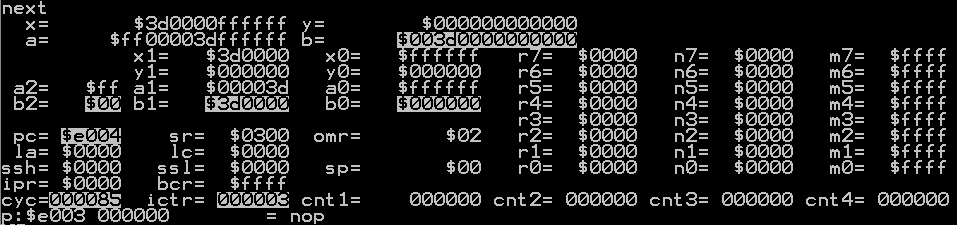
\includegraphics[width=\textwidth]{figs/ej1/3ra_i.png}
    \caption{Estado final de los registros (simulación).}
    \label{fig:ej1_simregs}
\end{figure}

\section{Ejercicio 2}

En el presente ejercicio se ejecutó el siguiente programa.

\lstinputlisting[language={[Motorola68k]Assembler}]{code/ej2.asm} 

Teniendo en cuenta que los registros parten desde los siguientes estados iniciales:

$$ a = \$00000000000000 $$
$$ b = \$00000000000000 $$
$$ x = \$000000000000 $$

\begin{table}[H]
\centering
\begin{tabular}{|c|c|c|}
\hline
\textbf{Instrucción} & \textbf{Cambios}                                                                                       & \textbf{Comentarios}                                                                                                                                                            \\ \hline
-                  & \begin{tabular}[c]{@{}c@{}}a = \$00000000000000\\ y = \$00000000000000\\ x = \$000000000000\end{tabular} & Carga inicial de valores                                                                                                                                                        \\ \hline
move \#\$caba00, x1         & x = \$caba00000000                                                                                  & \begin{tabular}[c]{@{}c@{}}Se modifica el valor del registro x1 con el valor caba00 \\ por lo que x resulta modificado al valor mostrado.\end{tabular}    \\ \hline
move x1,a                & a = \$ffcaba00000000                                                                                   & \begin{tabular}[c]{@{}c@{}}Se mueve x1 al registro a como el valor \\ caba empieza en 1 (base decimal) se completa \\ con ff (base hexadecimal) hacia adelante.\end{tabular}                                                                       \\ \hline
move x1, b1         & b = \$00caba00000000                                                                                   & \begin{tabular}[c]{@{}c@{}}En este caso el valor del registro x1 se guarda en el b1 \\por lo que b2 y b0 no se ven afectadas por este cambio \\(a diferencia de lo que hubiera pasado si \\guardábamos en el valor de x1 en b).\end{tabular} \\ \hline
\end{tabular}
\caption{Paso a paso de las instrucciones ejecutadas.}
\label{tab:ej2_inst_table}
\end{table}


En la tabla~\ref{tab:ej2_results} se muestra el estado final de los registros.

\begin{table}[H]
\centering
\begin{tabular}{|c|c|c|}
\hline
\textbf{Registro} & \textbf{Valor inicial} & \textbf{Valor final}  \\ \hline
x                 & \$000000000000         & \$caba00000000        \\ \hline
a                 & \$00000000000000       & \$ffcaba00000000      \\ \hline
b                 & \$00000000000000       & \$00caba00000000      \\ \hline
\end{tabular}
\caption{Estado inicial y final de los registros.}
\label{tab:ej2_results}
\end{table}

Se adjunta el estado final de los registros simulados.

\begin{figure}[H]
    \centering
    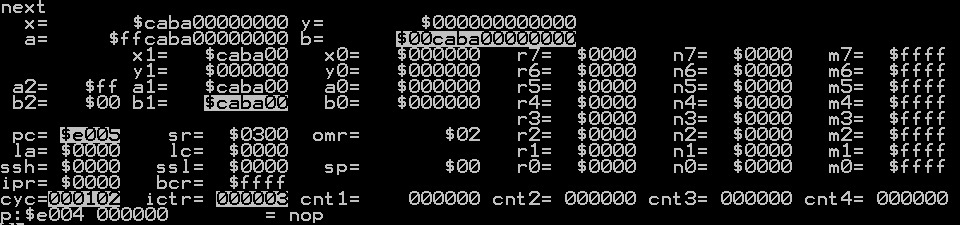
\includegraphics[width=\textwidth]{figs/ej2/ej2_2.jpeg}
    \caption{Estado final de los registros (simulación).}
    \label{fig:ej2_simregs}
\end{figure}

\section{Ejercicio 3}
En este ejercicio se corre el siguiente programa.

\lstinputlisting[language={[Motorola68k]Assembler}]{code/ej3.asm}


Teniendo en cuenta el siguiente estado inicial en los registros.

$$ a = \$00a00000000000 $$
$$ y = \$000000000000 $$
$$ ccr = \$00 $$

A continuación se muestra un desglose del programa, indicando aquellos registros que cambian a medida que este se ejecuta.

\begin{table}[H]
\centering
\begin{tabular}{|c|c|c|}
\hline
\textbf{Instrucción} & \textbf{Cambios}                                                                                                                  & \textbf{Comentarios}                                                                                                                                                                                                                          \\ \hline
-                  & \begin{tabular}[c]{@{}c@{}}a = \$00a00000000000\\ x = \$xxxxxxxxxxxx\\ y = \$000000000000\\ r7 = \$xxxx\\ ccr = \$00\end{tabular} & Carga inicial de valores.                                                                                                                                                                                                                     \\ \hline
move a1,x1           & \begin{tabular}[c]{@{}c@{}}x = \$a00000xxxxxx\\ ccr = \$00\end{tabular}                                                           & \begin{tabular}[c]{@{}c@{}}Carga de a1 (\$a00000) en x1.\end{tabular}                                                                                    \\ \hline
move a,y1            & \begin{tabular}[c]{@{}c@{}}y = \$7fffff000000\\ ccr = \$40\end{tabular}                                                           & \begin{tabular}[c]{@{}c@{}}Se interpreta al registro a como punto fijo.\\ a = 1,25. \\ Se produce overflow.\\ Se redondea y1 al máximo numero positivo representable.\\ En el CCR, se activa el bit \textit{Limit} (L=1) indicando lo anterior\end{tabular} \\ \hline
move a,r7            & \begin{tabular}[c]{@{}c@{}}r7 = \$ffff\\ ccr = \$40\end{tabular}                                                                  & \begin{tabular}[c]{@{}c@{}}Al mover el acumulador a a r7, se produce overflow.\\ Como r7 es entero, se interpreta a a como entero.\\ Se redondea r7 al máximo valor representable (\$ffff)\end{tabular}                                       \\ \hline
move a1,x0           & x = \$a00000a00000                                                                                                                & \begin{tabular}[c]{@{}c@{}}En este caso se realiza una operación de copia de registro.\\ No se interpreta el número como punto fijo.\end{tabular}                                                                                             \\ \hline
\end{tabular}
\caption{Paso a paso de las instrucciones ejecutadas.}
\label{tab:ej3_instructions}
\end{table}

En la tabla~\ref{tab:ej3_results} se muestra el estado final de los registros.

\begin{table}[H]
\centering
\begin{tabular}{|c|c|c|}
\hline
\textbf{Registro} & \textbf{Valor inicial} & \textbf{Valor final} \\ \hline
x                 & \$xxxxxxxxxxxx         & \$a00000a00000       \\ \hline
y                 & \$000000000000         & \$7fffff000000       \\ \hline
r7                & \$xxxx                 & \$ffff               \\ \hline
ccr               & \$00                   & \$40                 \\ \hline
\end{tabular}
\caption{Estado inicial y final de los registros.}
\label{tab:ej3_results}
\end{table}

Se adjunta el estado final de los registros simulados.

\begin{figure}[H]
    \centering
    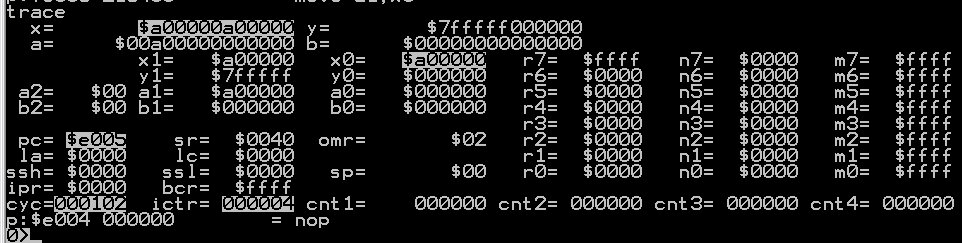
\includegraphics[width=\textwidth]{figs/ej3/3_4.png}
    \caption{Estado final de los registros (simulación).}
    \label{fig:ej3_simregs}
\end{figure}


\section{Ejercicio 4}

En el presente ejercicio se ejecutó el siguiente programa.

\lstinputlisting[language={[Motorola68k]Assembler}]{code/ej4.asm} 

A continuación, en la tabla \ref{tab:ej4_inst_table} se puede observar los cambios resultantes luego de ejecutar paso por paso cada una de las instrucciones del programa.


\begin{table}[H]
\centering
\begin{tabular}{|c|c|c|}
\hline
\textbf{Instrucción} & \textbf{Cambios}                                                                                       & \textbf{Comentarios}                                                                                                                                                            \\ \hline
-                  & \begin{tabular}[c]{@{}c@{}}a = \$00000123800000\\ b = \$ff000000ffffff\\ x = \$400000400000\end{tabular} & Carga inicial de valores                                                                                                                                                        \\ \hline
macr x0,x1,a         & a = \$00200124000000                                                                                   & \begin{tabular}[c]{@{}c@{}}Al registro a se le suma el producto de x0 y x1 y se lo redondea.\\ Luego, como en a0 resultaría \$800000, se redondea el resultado.\end{tabular}    \\ \hline
rnd b                & b = \$ff000001000000                                                                                   & \begin{tabular}[c]{@{}c@{}}Se redondea b.\\ Como b0 guardaba \$ffffff, en b1 resulta \$000001.\end{tabular}                                                                       \\ \hline
mpyr x1,x0,b         & b = \$00200000000000                                                                                   & \begin{tabular}[c]{@{}c@{}}En el registro b se guarda el producto de x1 y x0 y se lo redondea.\\ Como b0 resulta \$000000, el redondeo no influye en el resultado.\end{tabular} \\ \hline
\end{tabular}
\caption{Paso a paso de las instrucciones ejecutadas.}
\label{tab:ej4_inst_table}
\end{table}



Los valores finales de los registros a y b se observan en la tabla \ref{tab:ej4_a_b}.

\begin{table}[H]
\centering
\begin{tabular}{|c|c|c|}
\hline
\textbf{Registro} & \textbf{Valor Inicial} & \textbf{Valor Final} \\ \hline
a                 & \$00000123800000       & \$00200124000000     \\ \hline
b                 & \$ff000000ffffff       & \$00200000000000     \\ \hline
\end{tabular}
\caption{Valores iniciales y finales de los registros a y b.}
\label{tab:ej4_a_b}
\end{table}

Las instrucciones del programa fueron ejecutadas en el simulador, del cual se obtuvieron los resultados mencionados anteriormente. En las figuras \ref{fig:ej4_iniregs}, \ref{fig:ej4_insts}, \ref{fig:ej4_inst1}, \ref{fig:ej4_inst2} y \ref{fig:ej4_inst3} se muestran las capturas de la ejecución en el simulador.

\begin{figure}[H]
    \centering
    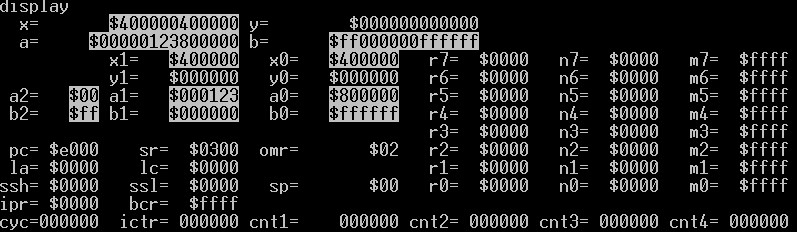
\includegraphics[scale=1]{figs/ej4/1.jpg}
    \caption{Carga inicial de los registros.}
    \label{fig:ej4_iniregs}
\end{figure}

\begin{figure}[H]
    \centering
    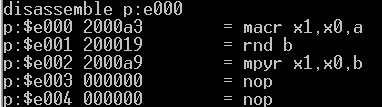
\includegraphics[scale=1]{figs/ej4/2.jpg}
    \caption{Carga de las instrucciones a ejecutar.}
    \label{fig:ej4_insts}
\end{figure}

\begin{figure}[H]
    \centering
    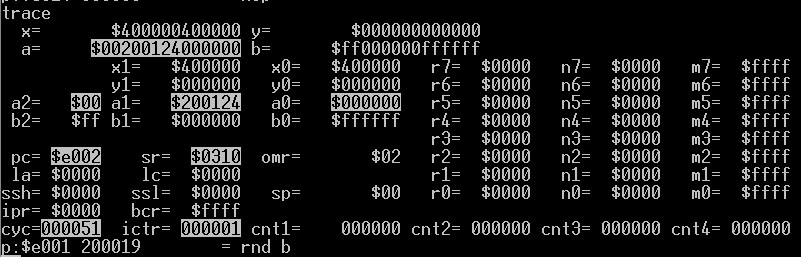
\includegraphics[scale=1]{figs/ej4/3.jpg}
    \caption{Primera instrucción ejecutada (macr x0,x1,a). }
    \label{fig:ej4_inst1}
\end{figure}

\begin{figure}[H]
    \centering
    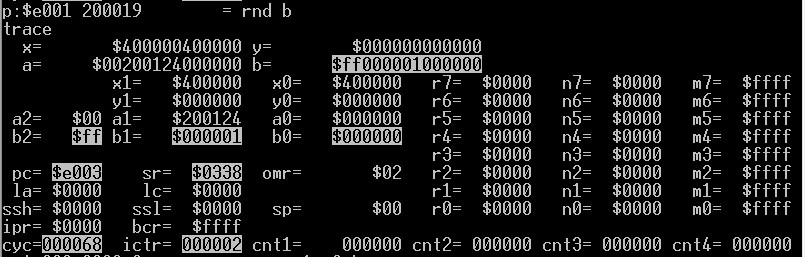
\includegraphics[scale=1]{figs/ej4/4.jpg}
    \caption{Segunda instrucción ejecutada (rnd b). }
    \label{fig:ej4_inst2}
\end{figure}

\begin{figure}[H]
    \centering
    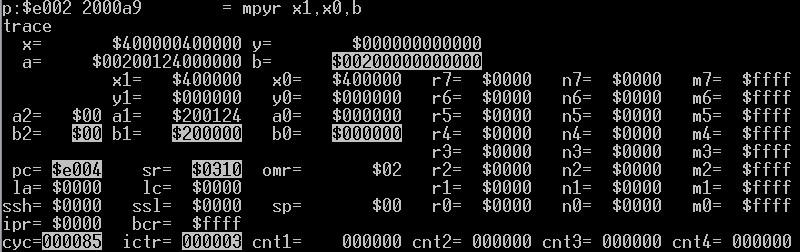
\includegraphics[scale=1]{figs/ej4/5.jpg}
    \caption{Última instrucción ejecutada (mpyr x0,x1,b). }
    \label{fig:ej4_inst3}
\end{figure}
\section{Ejercicio 5}
En el presente ejercicio se analiza la ejecución del siguiente código.

\lstinputlisting[language={[Motorola68k]Assembler}]{code/ej5.asm} 

\subsection{Status Register inicializado en \$0300}
Se imponen las siguientes condiciones iniciales a los registros.
$$ a = \$00000000000000 $$
$$ sr = \$0300 $$

Dentro de estas condiciones se destaca que el valor inicial del status register considera ambos bits de escala (S1, S0) en cero, por lo que no se produce escalamiento en el valor del acumulador. 

En la tabla~\ref{tab:ej5_instructions_a} se observa como se desarrolla la ejecución del programa en cuestión.

\begin{table}[H]
\centering
\begin{tabular}{|c|c|c|}
\hline
\textbf{Instrucción} & \textbf{Cambios}                                                           & \textbf{Comentarios}                                                                                                   \\ \hline
-                  & \begin{tabular}[c]{@{}c@{}}a = \$00000000000000\\ sr = \$0300\end{tabular} & Carga inicial de valores.                                                                                              \\ \hline
move \#\$400000,x0     & x0 = \$400000                                                              & \begin{tabular}[c]{@{}c@{}}Carga el valor inmediato en x0.\\ No hay cambios en el sr.\end{tabular}                     \\ \hline
add x0,a             & \begin{tabular}[c]{@{}c@{}}a = \$00400000000000\\ sr = \$0300\end{tabular} & \begin{tabular}[c]{@{}c@{}}Suma el valor de x0 en a.\\ a = 0,5.\\ El acumulador estaba inicializado en 0.\end{tabular} \\ \hline
add x0,a             & \begin{tabular}[c]{@{}c@{}}a = \$00800000000000\\ sr = \$0320\end{tabular} & \begin{tabular}[c]{@{}c@{}}Suma el valor de x0 en a.\\ a = 1.\\ Se activa el bit Extension (E=1).\end{tabular}         \\ \hline
\end{tabular}
\caption{Paso a paso de las instrucciones ejecutadas con sr=\$0300}
\label{tab:ej5_instructions_a}
\end{table}

La tabla~\ref{tab:ej5_results_a} refleja el estado final de los registros.

\begin{table}[H]
\centering
\begin{tabular}{|c|c|c|}
\hline
\textbf{Registro} & \textbf{Valor inicial} & \textbf{Valor final} \\ \hline
a                 & \$00000000000000       & \$00800000000000     \\ \hline
sr                & \$0300                 & \$0320               \\ \hline
\end{tabular}
\caption{Estado inicial y final de los registros con sr=\$0300}
\label{tab:ej5_results_a}
\end{table}

Se observa que luego de la ejecución del segundo \textit{add}, el acumulador toma el valor a = \$00800000000000. Esto surge de que se suma dos veces el valor 0,5, contenido en x0. De esta forma, el valor final del acumulador a es 1. Luego, el bit de extensión (E) del CCR se activa, indicando que se está usando la parte entera del acumulador. Esto sucede dado que en un número de punto fijo de 24 bits no es posible representar la unidad.


\begin{figure}[H]
    \centering
    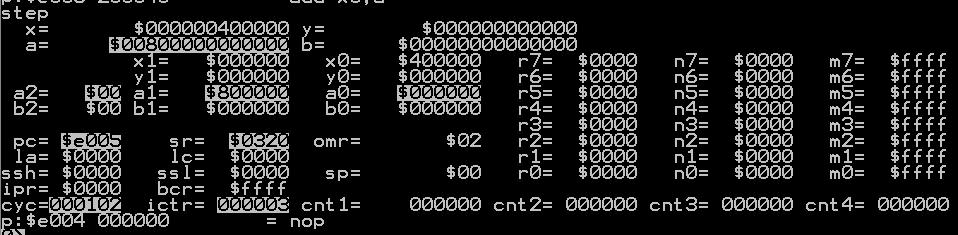
\includegraphics[width=\textwidth]{figs/ej5/ej5_3_a.png}
    \caption{Estado final de los registros con sr=\$0300 (simulación).}
    \label{fig:ej5_simregs_a}
\end{figure}

En la figura~\ref{fig:ej5_simregs_a} se observa el resultado de la simulación.


\subsection{Status Register inicializado en \$0700}
Se repite el análisis anterior, pero esta vez con las siguientes condiciones iniciales:

$$ a = \$00000000000000 $$
$$ sr = \$0700 $$

Esta vez se comienza con el bit de escalamiento S0 activo. Esta condición implica que se produce un shift aritmético hacia la izquierda de los acumuladores. De esta forma, se desplaza el punto fraccionario un lugar hacia la izquierda. Esto cambia la forma en la que el DSP computa los bits \textit{Unnormalized} y \textit{Extension} (U y E, respectivamente) del CCR.
\\
En la tablas~\ref{tab:ej5_instructions_b} y \ref{tab:ej5_results_b} se muestra el paso a paso en la ejecución de las instrucciones y los resultados, respectivamente.

\begin{table}[H]
\centering
\begin{tabular}{|c|c|c|}
\hline
\textbf{Instrucción} & \textbf{Cambios}                                                           & \textbf{Comentarios}                                                                                                      \\ \hline
-                  & \begin{tabular}[c]{@{}c@{}}a = \$00000000000000\\ sr = \$0700\end{tabular} & Carga inicial de valores.                                                                                                 \\ \hline
move \#\$400000,x0     & x0 = \$400000                                                              & \begin{tabular}[c]{@{}c@{}}Carga el valor inmediato en x0.\\ No hay cambios en el sr.\end{tabular}                        \\ \hline
add x0,a             & \begin{tabular}[c]{@{}c@{}}a = \$00400000000000\\ sr = \$0710\end{tabular} & \begin{tabular}[c]{@{}c@{}}Suma el valor de x0 en a.\\ a=0,5.\\ Se activa el bit Unnormalized del ccr (U=1).\end{tabular} \\ \hline
add x0,a             & \begin{tabular}[c]{@{}c@{}}a = \$00800000000000\\ sr = \$0700\end{tabular} & \begin{tabular}[c]{@{}c@{}}Suma el valor de x0 en a.\\ Se desactiva el bit Unnormalized del ccr (U=0).\end{tabular}       \\ \hline
\end{tabular}
\caption{Paso a paso de las instrucciones ejecutadas con sr=\$0700}
\label{tab:ej5_instructions_b}
\end{table}

\begin{table}[H]
\centering
\begin{tabular}{|c|c|c|}
\hline
\textbf{Registro} & \textbf{Valor inicial} & \textbf{Valor final} \\ \hline
a                 & \$00000000000000       & \$00800000000000     \\ \hline
sr                & \$0700                 & \$0700               \\ \hline
\end{tabular}
\caption{Estado inicial y final de los registros con sr=\$0700}
\label{tab:ej5_results_b}
\end{table}

De las tablas anteriores se concluye que el resultado en el acumulador a no cambió respecto del caso expuesto en la tabla~\ref{tab:ej5_results_a}. En contraposición, se aprecia que el comportamiento del CCR durante la ejecución es distinto que el de la tabla~\ref{tab:ej5_instructions_a}. Como se advirtió anteriormente, esto se debe al cambio en las condiciones de escalamiento impuestas por el nuevo valor inicial del status register, y en cómo estas afectan al cálculo de ciertos bits del mismo.

En este caso, al ejecutar el primer \textit{add}, se carga el valor \$00400000000000 en el acumulador a. Dado que ahora se trabaja con el punto fraccionario desplazado una posición hacia la izquierda, no se cumple la condición de normalización, activando el bit correspondiente en el CCR que indica que el acumulador no se encuentra normalizado. Al sumar nuevamente el valor de x0, pasa a cumplirse la condición de normalización y el bit U cambia su valor a 0.

Otra diferencia respecto al caso anterior es que luego de ejecutadas las instrucciones, no se activa el bit de extensión del CCR. Nuevamente, esto se debe al desplazamiento hacia la izquierda del punto fraccionario. En este caso, esta modificación resulta en que el valor final del acumulador sea 0,5 en lugar de 1, lo cual implica que no se está haciendo uso de la parte entera del mismo.


\begin{figure}[H]
    \centering
    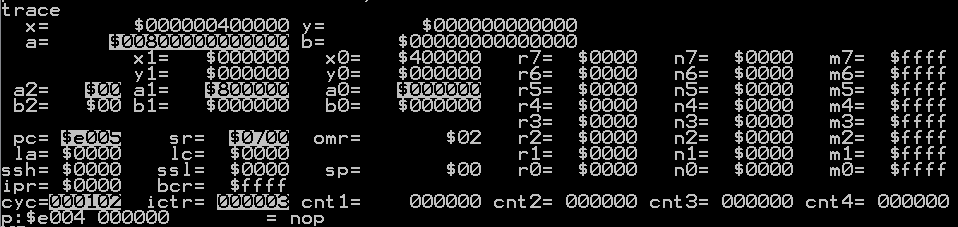
\includegraphics[width=\textwidth]{figs/ej5/ej5_3_b.png}
    \caption{Estado final de los registros con sr=\$0700 (simulación).}
    \label{fig:ej5_simregs_b}
\end{figure}

La figura~\ref{fig:ej5_simregs_b} muestra el resultado de la simulación realizada.

\section{Ejercicio 6}

En el presente ejercicio se ejecutó el siguiente programa.

\lstinputlisting[language={[Motorola68k]Assembler}]{code/ej6.asm} 

Teniendo en cuenta que los registros parten desde los siguientes estados iniciales:

$$ a = \$00000000000000 $$
$$ x = \$0c0000600000  $$
$$ r0 = \$0000 $$


\begin{table}[H]
\centering
\begin{tabular}{|c|c|c|}
\hline
\textbf{Instrucción} & \textbf{Cambios}                                                                                       & \textbf{Comentarios}                                                                                                                                                            \\ \hline
-                  & \begin{tabular}[c]{@{}c@{}}a = \$00000000000000\\ x = \$0c0000600000\\ r0 = \$0000\end{tabular} & Carga inicial de valores                                                                                                                                                        \\ \hline
add x1,a         & a = \$000c0000000000                                                                                  & \begin{tabular}[c]{@{}c@{}}se suma a con el valor almacenado en x1 \\ y se guarda el resultado de la suma en a.\end{tabular}    \\ \hline
\begin{tabular}[c]{@{}c@{}}rep \#\$a \\ norm r0,a         \end{tabular}    & a = \$00600000000000                                                                                   & \begin{tabular}[c]{@{}c@{}}En esta instrucción se realiza en un loop 10 veces \\ la siguiente instruccion en este caso la instrucción norm \\ para ver qué ocurre dentro del loop referirse a la tabla \ref{ej6_loop_table} \end{tabular}                                                                       \\ \hline
add x0,a         & a = \$00c00000000000                                                                                   & \begin{tabular}[c]{@{}c@{}}se suma x0 al registro a, de esta manera lo que termina \\sucediendo es un shifteo a derecha debido a que se \\ terminan  sumando 2 números iguales. Luego de la suma \\ los bits E, U y Z valen como se indica en la tabla \ref{ej6_EUZ}.\end{tabular} \\ \hline
\end{tabular}
\caption{Paso a paso de las instrucciones ejecutadas.}
\label{tab:ej6_inst_table}
\end{table}


\begin{table}[H]
\centering
\begin{tabular}{|c|c|c|c|c|c|}
\hline
\textbf{Iteración}  & \textbf{E} & \textbf{U} & \textbf{Z} & \textbf{Acción} & \textbf{Valor del acumulador a} \\ \hline
1   &  0   & 1  &  0  & ASL & \$00 180000 000000        \\ \hline
2   &  0   & 1  &  0  & ASL & \$00 300000 000000        \\ \hline
3   &  0   & 1  &  0  & ASL & \$00 600000 000000        \\ \hline
4   &  0   & 0  &  0  & NOP & \$00 600000 000000        \\ \hline
5   &  0   & 0  &  0  & NOP & \$00 600000 000000        \\ \hline
\end{tabular}
\caption{Pasos internos del Loop, luego del paso 5 se repiten las filas hasta la iteración numero 10}
\label{ej6_loop_table}
\end{table}

\begin{table}[H]
\centering
\begin{tabular}{|c|c|c|}
\hline
\textbf{E} & \textbf{U} & \textbf{Z} \\ \hline
1                 & 1       & 0     \\ \hline
\end{tabular}
\caption{Valores de los bits E, U y Z al finalizar la ejecución.}
\label{ej6_EUZ}
\end{table}



\section{Ejercicio 7}
En el presente ejercicio se analiza la ejecución del siguiente código.

\lstinputlisting[language={[Motorola68k]Assembler}]{code/ej7.asm}

Del código se destaca que se inicializa al \textit{status register} con el valor \$0800. Del manual del DSP 56000 de Motorola se extrae que se activa el bit S1, lo que configura el \textit{scaling mode} en \textit{Scale Up}, lo cual produce un corrimiento del punto fraccionario hacia la derecha, aumentando la parte entera en 1 bit. 

\begin{table}[H]
\centering
\begin{tabular}{|c|c|c|}
\hline
\textbf{Dirección} & \textbf{Mapa X (origen)} & \textbf{Mapa Y (destino)} \\ \hline
\$0000             & \$10fedc                 & \$21fdb8                  \\ \hline
\$0001             & \$210fed                 & \$421fda                  \\ \hline
\$0002             & \$4210fe                 & \$7fffff                  \\ \hline
\$0003             & \$84210f                 & \$800000                  \\ \hline
\$0004             & \$d84210                 & \$b08420                  \\ \hline
\$0005             & \$fb8421                 & \$f70842                  \\ \hline
\end{tabular}
\caption{Estado de la memoria luego de correr el programa.}
\label{tab:ej7_mem}
\end{table}

En la tabla~\ref{tab:ej7_mem} se muestra el resultado de la ejecución del programa, donde se puede observar el efecto del \textit{Scale Up} ya que las posiciones de memoria en Y surgen de realizar un shift aritmético a izquierda sobre las posiciones de memoria en X, exceptuando las posiciones \$0002 y \$0003 ya que en las mismas al cargarse sobre el acumulador A e interpretarse como numero de punto fijo corresponden a números, en modulo, mayor a 1, por lo cual al intentar realizar el movimiento del acumulador al espacio de memoria actuará el limitador.

\begin{figure}[H]
    \centering
    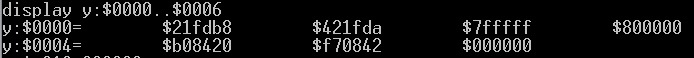
\includegraphics[width=\textwidth]{figs/ej7/1.jpeg}
    \caption{Estado final de la memoria (simulación).}
    \label{fig:ej7_mem}
\end{figure}

\begin{figure}[H]
    \centering
    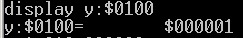
\includegraphics[width=0.5\textwidth]{figs/ej7/2.jpeg}
    \caption{Estado final de la memoria Y:\$0100 (simulación).}
    \label{fig:ej7_y100}
\end{figure}

En la figura~\ref{fig:ej7_y100} se aprecia que el valor final de la posición de memoria Y:\$0100 es 1. Observando el programa, se concluye que esta posición de memoria puede estar siendo empleada como flag para indicar si en algún momento de la ejecución existió un redondeo. 
\section{Ejericicio 8}

En este ejercicio se implementó la subrutina \textit{vect\_max}, la cual recibe por registros punteros a dos vectores \textit{A} y \textit{B}, los compara y devuelve en \textit{B} aquellos valores de mayor valor absoluto. 

Se reciben los punteros a los vectores A y B en los registros $r_0$ y $r_4$, respectivamente, correspondiendo  $r_0$ a una región de memoria en X, y $r_4$ a una región de memoria en Y. En el registro $n_0$ se recibe el tamaño de los vectores a comparar.
\\
\\
Se propone el siguiente \textit{main} de prueba.

\lstinputlisting[language={[Motorola68k]Assembler}]{code/ej8.asm}

En la figura~\ref{fig:ej8_results} se muestra el resultado de simular el código propuesto.

\begin{figure}[H]
    \centering
    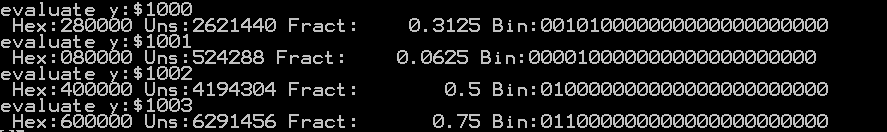
\includegraphics[width=\textwidth]{figs/ej8/ej8_result.png}
    \caption{Estado final del vector B (Simulación}.
    \label{fig:ej8_results}
\end{figure}

\end{document}
